After the research of the current state of the art explained in the previous section we proceed with the following rosearch questions, that will be addressed during the first part of the PhD as well.
In order to answer RQ2 while explaining our proposed process we divided this part into different tasks.
First, we defined the software architecture that defines our system.
Then, we will implement configuration facilities that enables the customization of the different components that compose the architecture.
Finally, we will develop the software platform where the previous work is implemented.

\subsection{Software architecture}

Our software architecture, Self-adaptive dEcentralised Robotic Architecture (SERA) is already defined.
As its name indicates, it supports a real-time decentralized robot coordination to accomplish missions with teams of robots. 
Furthermore, it is self-adaptive, responding to different changes by computing new strategies to achieve the desired goals.
SERA is inspired by and extends concepts of existing proposals for robot software architectures from the literature. 
Specifically, we inspected architectures identified by a mapping study of Ahmad et al.~\cite{Ahmad201616}, which investigated software architectures for robotics systems to identify and analyze the relevant literature based on 56 peer-reviewed papers.
The aforementioned architecture is three layers architecture that is strongly influenced by the well-known work of Kramer and Magee~\cite{kramer}.
It has the same structure, but we also added a new item that works as a central station.
It is important to remark that the aim of our project is to build a system that can be easily used by not technical users, so we had to define a way for them to command the missions to the robotic team.
The central station is just used during design-time in order to allocate a graphical interface to be used by a final user.

We defined SERA by first conceiving an architecture for a single robot. 
It means that all components, interfaces and units were defined for a single robot architecture. 
Then, we extended and refined it in order to iteratively extend and refine the architecture towards enabling communication among robots and collective adaptations. 
Thus, all the robots have a instantiation of the reference architecture but are also able to communicate and share information with the rest of the team, making possible the collective adaptation. 

SERA was already tested during an Integration Meeting of the project, where it demonstrate that can support the performance of a robot achieving different complex missions ---i.e. collaborative transportation with an human being, autonomous driving in a dynamic environment.

%\begin{figure*}[!t]
%\begin{center}
%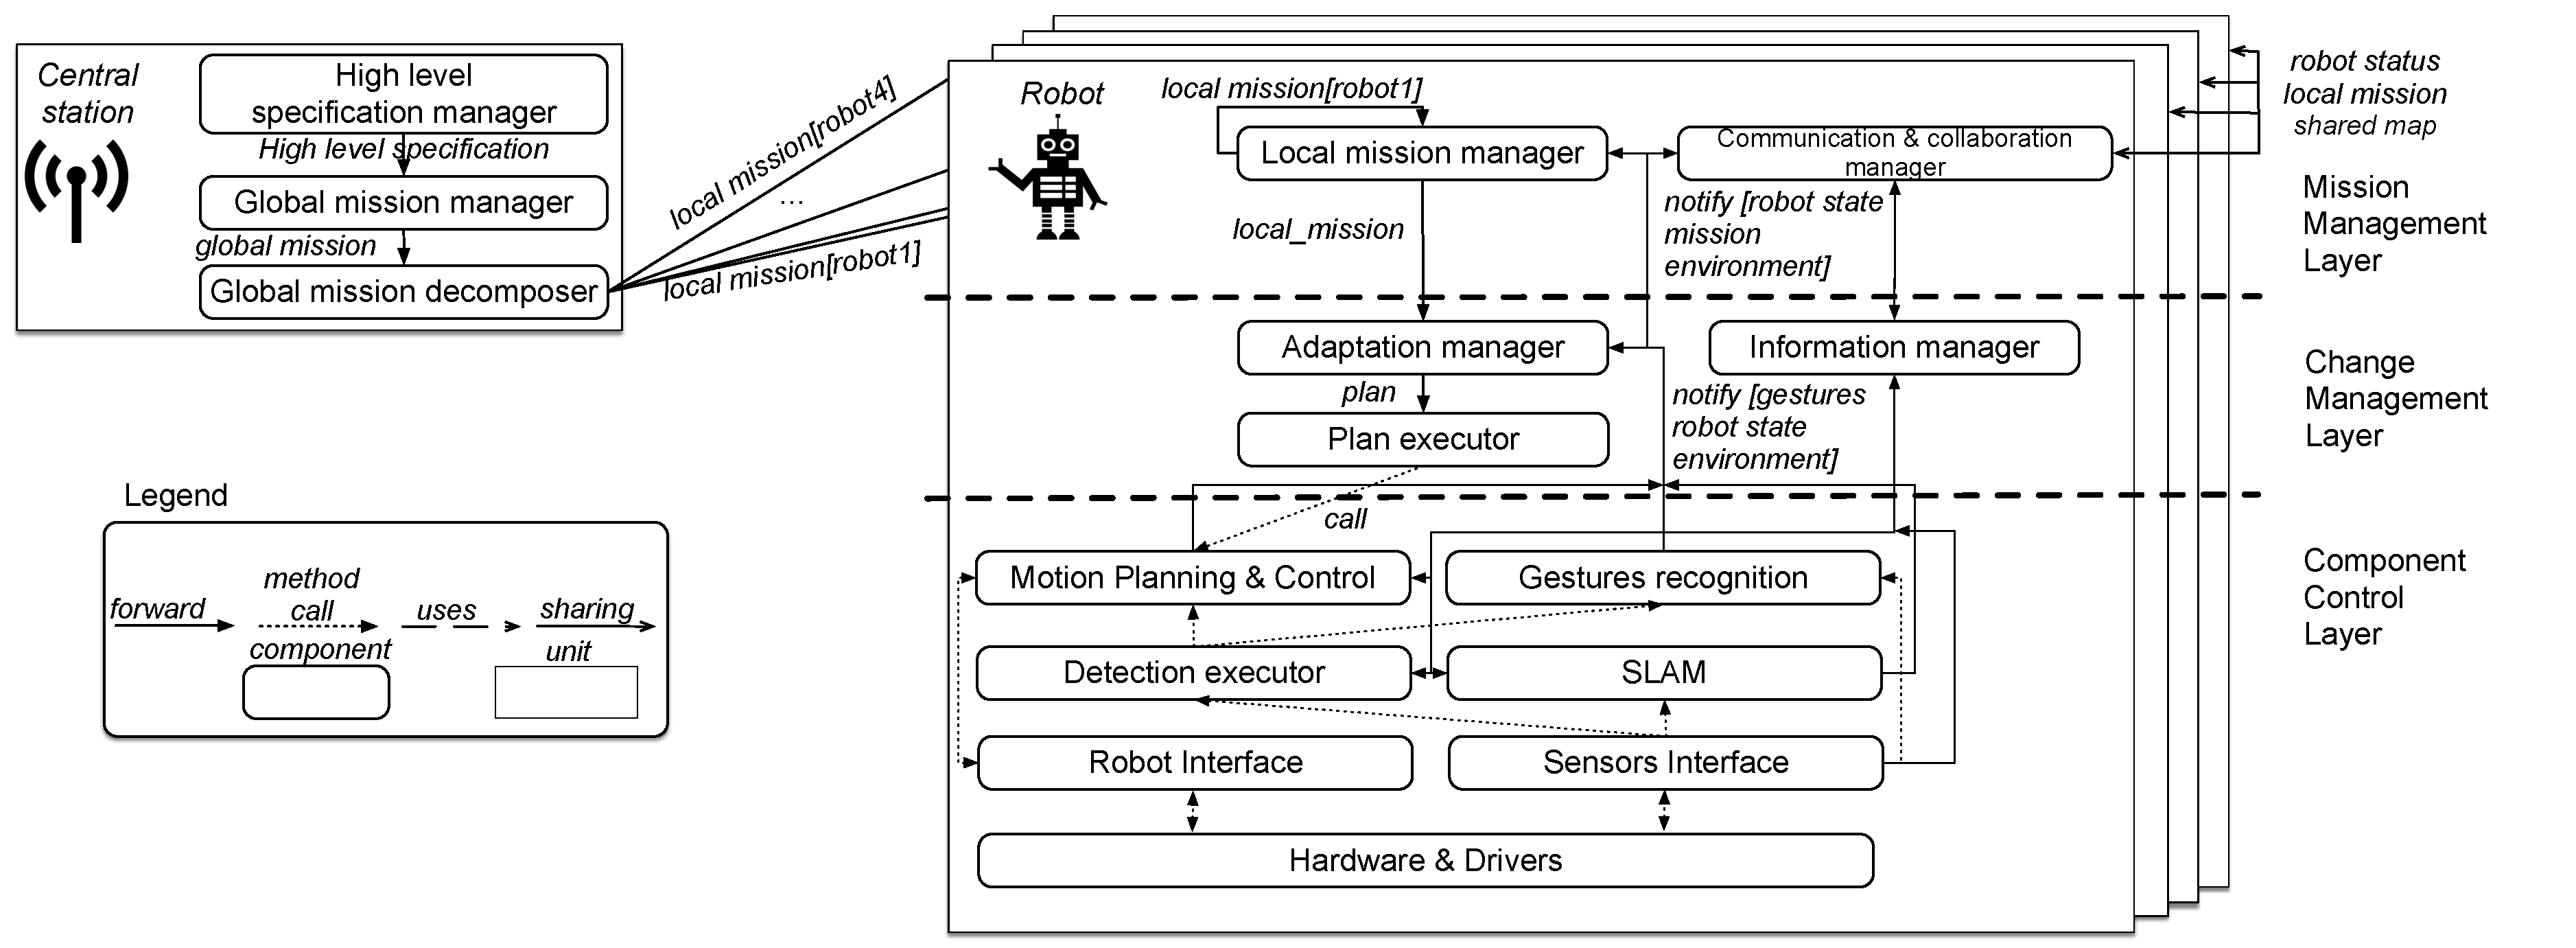
\includegraphics[width=1\linewidth]{Figures/InstanceMultiRobot_Graffle.pdf}
%\caption{Software architecture.}
%\label{fig:arch}
%\end{center}
%\end{figure*}

\subsection{Configuration facilities}

Since the components of our architecture are exchangeable our next short-term goal is to define configuration facilities that can be applied to our system depicted in the architecture.
It will allow to our applications to support two things:
\begin{enumerate}
\item Being customizable at design-time, so we can configure its components based on the requirements of our context (i.e. hardware installed in each robot, environment where they will be deployed, etc.)
\item To self-adapt or self-configure at run time, so each robot can apply changes in its configuration based on emergent events of the environment or failures of their system.
\end{enumerate}

In order to do so we will implement pluginlib~\footnote{http://wiki.ros.org/pluginlib}, a package that uses the ROS build infrastructure and provides tools for writing and dynamically loading plugins.

\subsection{Software platform}

As explained before, the Software platform will integrate the Software architecture and all the tools and software created by developers and also the configuration facilities.
Regarding the architecture, SERA follows the component-based style, so the main robotic functionalities are encapsulated in different modules or "components".
The platform is also a collection of such components, a kind of library.
All this components are developed abstracting the communication capabilities since we rely on the interfaces defined in the architecture.
It not only significantly reduces the complexity of the code but also triggers the modularity of our system making possible exchanging the components that conform our architecture.

We not only plan to control the performance of the system that is running in each robot but also its behaviour.
Thus, the usage of high-level behavior engine, flexibly applicable to numerous systems and scenarios is mandatory.
FlexBe~\cite{Schillinger2016} not only provides a way of defining the behaviour of the robot in different scenarios (as of the study cases) by means of a work flow, but also a graphical interface that simplifies enormously this task.
FlexBe encapsulates functionalities of the robotic application, as our architecture does within components, and provides a way of orchestrate them so we keep the modularization of our system.
As with ROS, an instantiation of FlexBe will be deployed in every robot.
The integration of FlexBe is driven for the necessity of a software development methodology as MDE in our project.
It improves the modularity, variability and reusability of our system facilitating the development of the software for animating robotic systems through the creation of reusable robot building blocks with well-defined interfaces and properties.

Finally, in order to communicate each robot with its teammates we implemented an approach based on ROS+REST.
So, using a suitable component that works as an interface we are able to send messages in form of services between robots.
In this way, each robot has an instance of ROS running in their own local environment so we can deploy a whole team of robots avoiding a central master node and the problems related with this approach (i.e. bottleneck issues, less robustness facing failures of a node, etc.), specially working with the ROS middleware.

